% !TEX root = ../main.tex



\item\pt{6}\begin{minipage}[t]{.6\linewidth}
	 De nevenstaande figuur toont een stel voorwerpen die met elkaar verbonden zijn met massaloze touwen die wrijvingsloos bewegen over katrollen. Het voorwerp met massa $2m$ schuift over een horizontale tafel. $m$ is gelijk aan \SI{2,0}{kg}. Alle voorwerpen hebben een versnelling van \SI{1,5}{m/s^2}. 
\end{minipage}
\hfill
\begin{minipage}[t]{.37\linewidth}
	\raisebox{1ex-\height}{%
		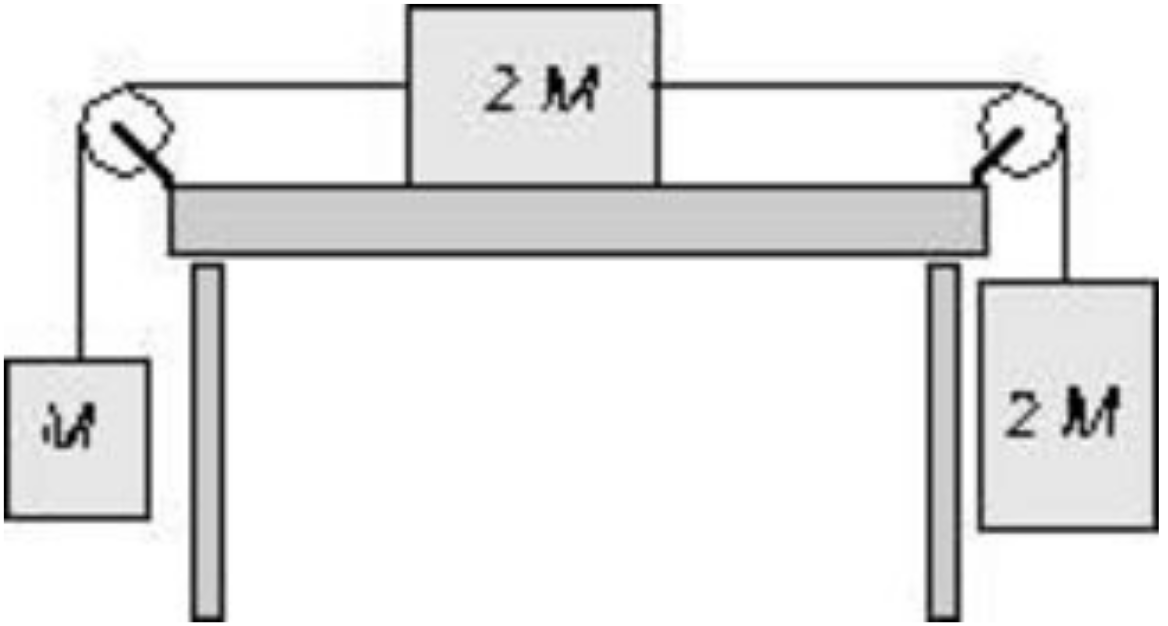
\includegraphics[width=\textwidth]{drieblokken_2}%
		} 
\end{minipage}

\begin{enumerate}
	\item Teken alle krachten op de blokken.
	\item Bepaal de grootte van de wrijvingskracht op het blok dat over de tafel glijdt.
\end{enumerate}



\begin{oplossing}
	\includepdf[pages={1},scale=.8]{./opl/VFO_9_8.pdf}
\end{oplossing}